\documentclass{bioinfo}
\copyrightyear{2020} \pubyear{2020}

\access{Advance Access Publication Date: Day Month Year}
\appnotes{Manuscript Category}

\begin{document}
\firstpage{1}

\subtitle{Sequence analysis}

\title[short Title]{AttCRISPR : an spacetime interpretable model for sgRNA efficiency prediction
}
\author[Sample \textit{et~al}.]{Corresponding Author\,$^{\text{\sfb 1,}*}$, Co-Author\,$^{\text{\sfb 2}}$ and Co-Author\,$^{\text{\sfb 2,}*}$}
\address{$^{\text{\sf 1}}$Department, Institution, City, Post Code, Country and \\
$^{\text{\sf 2}}$Department, Institution, City, Post Code,
Country.}

\corresp{$^\ast$To whom correspondence should be addressed.}

\history{Received on XXXXX; revised on XXXXX; accepted on XXXXX}

\editor{Associate Editor: XXXXXXX}

\abstract{\textbf{Motivation:} More and more higher specificities Cas9 variants are developed to avoid the off-target effect, which bring a significant volume of experimental data. 
Conventional machine learning performance poorly on these datasets, while model based on deep learning are often lack of interpretability, which makes it difficult for researchers to understand its decisions. 
Moreover, neither the deep learning based model with existing structure can not satisfy enough precision at such huge datasets.\\
\textbf{Results:} To overcome it, we design and implement AttCRISPR, a deep learning based model to predict the on-target activity. 
Our model was trained and tested on the biggest dataset, DeepHF dataset, as far as we know for performance evaluation. 
AttCRISPR achieves the best performance on DeepHF dataset, yielding an average spearman value of 0.99\%, 0.99\%, 0.99\% (corresponding to WT-SpCas9, eSpCas9(1.1), SpCas9-HF1) under tenfold shuffled validation. 
In addition, another advantage of AttCRISPR over other well-perform methods is that it is intrinsic interpretable and does not rely on other post hoc explanations techniques. 
In this paper, We design a set of algorithm to reveal the biological significance of the decision maked by AttCRISPR from the global and local perspectives at sgRNA overall level and nucleotide level.\\
\textbf{Availability:} The example code are available at \href{https://github.com/South-Walker/AttCRISPR}{https://github.com/South-Walker/AttCRISPR}\\
\textbf{Contact:} \href{xlm@xiaoliming96.com}{xlm@xiaoliming96.com}\\
\textbf{Supplementary information:} Supplementary data are available at \textit{Bioinformatics}
online.}

\maketitle

\section{Introduction}

Clustered regularly interspaced short palindromic repeats (CRISPR) / CRIPSR associated protein 9 (Cas9) systems is preferred over other biological research and human medicine technologies now, beacuse of it's efficiency, 
 robustness and programmability.  Cas9 nucleases can be directed by short guide RNAs (sgRNAs) to introduce site-specific DNA double-stranded breaks in target, 
 so to enable editing site-specific within the mammalian genome \citep{jinek2012a,cong2013multiplex,mali2013rnaguided}. CRISPR/Cas9, to a large extent, has developed genetic therapies at the cellular level, 
 while there are still severe medical disadvantage even now which has greatly hindered the further clinical application of the CRISPR/Cas9 systems. 
 One of these disadvantage is due to point mutations caused by off-target effects \citep{rubeis2018risks,kang2016introducing,ishii2017reproductive,liang2015crispr/cas9-mediated}. 
 To overcome this disadvantage, a solution is to engineer CRISPR / Cas9 with higher specificities. 
 That's why more and more higher specificities Cas9 variants, such as enhanced SpCas9 (eSpCas9(1.1)), 
 Cas9-High Fidelity (SpCas9-HF1) \citep{ishii2017reproductive,slaymaker2016rationally}, hyper-accurate Cas9 (HypaCas9) \citep{kleinstiver2016high-fidelity}, 
 been developed and bring a significant volume of experimental data, that is to say researchers have to face the difficulty of analyzing such huge and heterogeneous data.

The activity of chosen sgRNA sequence determines the success of genome editing, however distinctly fluctuant behaviors have been observed for the performance of different sgRNAs, even in the same Cas9 system.
 Some optimum sgRNAs can hit almost all targers alleles, while anothers don't even show activity \citep{wang2019optimized}.
 This fact indicates that it's meaningful to explore an efficient approaches to guide sgRNA design. 


In practice, there have been a number of application and toolkit applied in this task. In the earlier studies, methods in silico are categorized into three types: 
 (1) alignment-based, (2) hypothesis-driven and (3) learning-based \citep{chuai2018deepcrispr}. 
 Recently we noticed that the last type of method seems to be getting more attention because of huger and huger data set \citep{liu2019computational}. 

Learning-based method, which designed to predict the on-target activity (or off-target probability) of sgRNAs, 
 is essentially a computational model built by machine learning algorithm, not only conventional machine learning but also deep learning algorithm. 
 In general, the single or multiple base sequences (vary according to the task) and biological features are represented as a multi-dimensional vector $X\in\mathbb{R}^d$, 
 and $d=l+b$, where $l$ refers to the length of base sequences and $b$ refers to the number of biological features, these methods can be represented as
\begin{equation}
\text{\it y}=Score(\it X)\label{eq:01}
\end{equation}
 where $Score(\cdot)$ depends on the algorithm being selected, and $y$ denotes the predicted value.
 Some studies on HT\_ABE and HT\_CBE have shown that deep learning based models often outperformed conventional machine learning, when the number of sgRNAs in the data set reached a certain level \citep{Song2020,kim2018deep,kim2019spcas9}. 
 Per contra, conventional machine learning algorithms, such as linear regression, logistic regression and the decision tree, are often more interpretable due to the fewer parameters and clearer mathematical assumptions. 
 In short, what was needed for developer is to trade-off accuracy and interpretability. 
 \citeauthor{MuhammadRafid2020} consider deep-learning-based models as black boxs and believe they lack interpretability, 
 motivated by the empirical assertion, they turn to build a model based conventional machine learning to compete with state of the art deep learning models \citep{MuhammadRafid2020}. 
 On the other hand, input perturbation based feature importance analysis become a preferred components to reveal the importance of features in deep learning models. 
 \citeauthor{Liu2019} use a sliding window of length 2 to extract dimeric as input and rank the position of dimeric by contribution to final output \citep{Liu2019}. 
 One regret is that subject to the processing of the input sgRNA sequence, their analysis can not exactly on the nucleotide class. 
 Further, SHAP, one of the most prominent of model explain techniques, has been widely used to understand the decision made by the model. 
 \citeauthor{wang2019optimized} develope DeepHF, a deep learning based model, and use Deep SHAP to revealed nucleotide contributions \citep{wang2019optimized}. 
 Deep SHAP is a compositional approximation of SHAP values since it is challenged to computate SHAP values exactly, especially for a complex deep neural networks \citep{lundberg2017a}. 
 In our understanding, the method based on input perturbation often requires better generalization ability of the model (even for artificial ridiculous noise data). 
 Moreover, recent work indicates that model explain techniques, which based post hoc explanations techniques and input perturbations, could be fooled to generate meaningless explanations instead of reflecting the underlying biases \citep{slack2019fooling}, 
 in other word, they could be unreliable and misleading, even on model with excellent performance. 
 In addition, as far as we know, all the interpretable deep learning models today can only analyze the preference of on-target activity (or off-target probability) on specific nucleotide species and position 
 for example, the G adjacent to PAM has a positive effect on sgRNA activity as \citeauthor{wang2019optimized} report, 
 which we'll call the first-order preference in our paper, due to it's similar to the total differential of $y$ in Equation~(\ref{eq:01}) as following
\begin{equation}
dy = \sum^{d}_ia_idx_i\label{eq:02}
\end{equation}
\begin{equation}
a_i=\frac{\partial}{\partial x_i} Score(X)\label{eq:03}
\end{equation}
 where $x_i$ denotes the $i$-th dimension of the vector $X$, 
 $a_i$ indicates how dramatically the function changes as $x_i$ changes in a neighborhood of $X$. 
 Similarly the first-order preference indicates how dramatically the function changes as $x_i$ changes, in other word, the importance of $x_i$.
 However they didn't analyzed the preference for position $i$ nucleotide at the overall level, 
 which we'll call the second-order preference in our paper due to its calculation is based on first-order preference, 

 Specifically, we use a vector $A_i$ to build the first-order original preference at position $i$ within sgRNA sequence, then
 define $\tilde{A}$ as the first-order combine preference matrix (or just first-order preference), which means $\tilde{A}$ can be expressed linearly by $A$ as follow
\begin{equation}
\tilde{A}=BA\label{eq:04}
\end{equation}
where the weight matrix $B\in\mathbb{R}^{l\times l}$ is learned through attention mechanism. 
Then the predicted value can be expressed as
\begin{equation}
y=\sum_i^lW_i\tilde{A}_i\cdot {X_e}_i\label{eq:05}
\end{equation}
 where $W\in\mathbb{R}^l$ denotes a non-negative weight vector, $W_i$ denotes the weight of the $i$-th position, ${X_e}_i$ denotes the embedding vector of the nucleotide at $i$-th position.
 Assume that in Equation~(\ref{eq:04}) the first-order original preference at each position is relatively independent and weight matrix $B$ is independent of any first-order original preference, 
 then the total differential of the first-order preference at $i$-th position $\tilde{A}_i$ could be written as
\begin{equation}
d\tilde{A}_i=\sum_j^lB_{ij}EdA_j\label{eq:07}
\end{equation}
where $E$ is the identity matrix, and we call $B$ as the second-order preference matrix, 
it can explain how a particular pattern containing two nucleotides affects the base sequence, 
for example, how does the degree of preference for the G adjacent to PAM be affected by a T at 2 bases upstream?

\begin{figure}[!tpb]%figure2
    \centerline{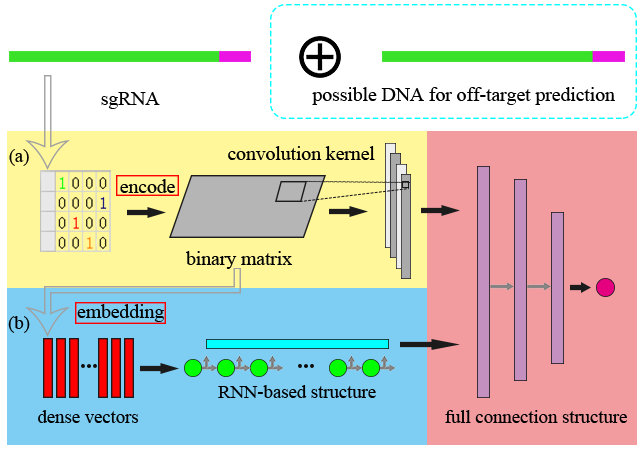
\includegraphics[width=86mm]{category.png}}
    \caption{Two categories of the deep learning models used in sgRNA related task. 
    (a) Model work in spatial domain. 
    In spatial domain, the base sequence is encoded into a binary matrix (or a binary image). 
    Since convolution has great advantages in extracting spatial features, the convolutional neural network is an excellent tool in spatial domain. 
    (b) Model work in temporal domain. 
    In temporal domain, the base sequence (represented by the binary matrix) is embedded into a sequance of high-dimensional vector, 
    in which the recurrent neural network perform better.
    In addition, we note that the last layers of neural network are usually full connection structure (not necessarily), 
    which greatly increases the difficulty of understanding the decisions of model.
    }\label{fig:01}
\end{figure}
 The previous work (even based on conventional machine learning algorithms with high interpretability) 
 was limited to dimers which can only work on the adjacent base pairs \citep{Liu2019} 
 or have to perform complex feature engineering \citep{MuhammadRafid2020}.
 In light of the above, we believe it is essential to develope a model which can not only match deep learning based model in performance, 
 but also be comparable to conventional machine learning algorithms in interpretability.

Deep neural network has shown its power in the study of CRISPR/Cas9 and its improved Systems \citep{liu2019computational}. 
 Most of the deep neural network existing are the combination of recurrent neural network (RNN), convolutional neural network (CNN), fully connected neural network (FNN), and their variants. 
 As Figure~1\vphantom{\ref{fig:01}} show,  
 We found that the deep learning models used in sgRNA on-target activity (even for off-target effect) prediction tasks in recent years can be divided into the following two categories according to the encoding approach of the sgRNA sequence (sgRNA-DNA sequence pair, for off-target effect prediction):

\begin{enumerate}
    \item Methods in spatial domain. 
    Some previous studies have used model based CNN to predict gRNA on-target activity or off-target effects \citep{lin2018off-target,kim2018deep,chuai2018deepcrispr}. 
    They process sgRNA base sequence inputs with the help of one-hot encoding idea. 
    In other words, they regard it as two-dimensional image data, and use convolution layer to extracte potential features in spatial domain, 
    It is worth noting that \citeauthor{zhang2020c-rnncrispr:} adds bidirectional gated recurrent unit (BGRU, in short), a RNN variant, after pooling layer of classic CNN network \citep{zhang2020c-rnncrispr:}. 
    Our explanation is that BGRU assists CNN to extract spatial features in one dimension, under this belief it belong to this category. 
    \item Methods in temporal domain. 
    Although RNN-based network have been shown effective to improve the performance of the model with temporal sequential input, especially in natural language processing and sequential recommendation\citep{huang2018improving}, 
    RNN be not used for gRNA activity prediction, until recently \citep{wang2019optimized,liu2020deep,Liu2019}. 
    They consider the nucleotides(can also dimer or polymer) in the sgRNA sequence as word, and the sgRNA sequence itself as a sentence (from 5' to 3'), then a trainable matrix (could be either supervised or unsupervised) is used to project the word to the dense real-valued space. 
    This technology is called embedding, which generates the base embedding. RNN further encoding the base embedding into a sequence of hidden state vector. 
    Specially, \citeauthor{Liu2019} use RNN and CNN in parallel to extract features in base embedding \citep{Liu2019}. 
    However, base embedding is not spatially interpretable (different from one-hot encode), and they have no way to further explore the correlation between CNN and RNN output. 
    Almost all RNN based models used in sgRNA on-target activity or off-target effect flatten the hidden state vector into a one-dimensional vector as the input of the fully connected layer. 
    It is a pity that the temporal sequential dependency of hidden state vector are rarely noticed. 
    To summarise, RNN has limited representation power in capturing spatial feature. Furthermore, hidden state vector representation is usually hard to understand and explain.
\end{enumerate}

Attention mechanism has demonstrated its power in Natural Language Processing, Statistical Learning, Speech and Computer Vision \citep{chaudhari2019an}. 
 It makes model tends to focus selectively on parts of the input which is help in performing the task effectively. 
 Previous observation have shown that Cas9 preferentially binds sgRNAs containing purines but not pyrimidines \citep{wang2014genetic} and multiple thymine in the spacer impairing sgRNA activity \citep{wu2014genome-wide}, 
 that is to say some specific nucleotide and base position need more attention compared to others. 
 The above is the premise of introducing attention mechanism. Strictly speaking, we are not the first to bring attention mechanisms into this field. 
 The most similar approach to ours is the work based on transformer by \citeauthor{Liu2019}. 
 They use transformer, a components based on attention mechanism, instead of RNN to improve the ability of temporal feature extraction, 
 hence, enhance the performance of their model \citep{Liu2019,vaswani2017attention}. 
 In our work,the interpretability benefit from attention mechanism is more focused.
 In this paper, our main contributions are as follows:\vspace*{1pt}
\begin{itemize}
    \item Present a novel deep-learning-based model, which can extract potential feature representation of sgRNA sequence in both spatial and temporal domain parallelly. 
    Finally, the ensemble learning method is used to combine the two to achieve better performance than other models.
    It doesn't belong to any of the above categories of existing approaches.
    \item Introduce attention mechanism into our model. 
    As a result, It does not need post hoc explanations techniques based on input perturbation to explain itself. 
    It is intrinsic interpretable in both temporal and spatial domains.
    In the spatial domain it's at the nucleotide level, in our word, first-order preference, 
    while at the overall level in the temporal domain, in our word, second-order preference. 
    Thus, it is transformed from a black box to an intrinsically interpretable model with the performance of deep learning based model. 
    \item Throught abation analysis and testing a series of possible network structure, 
    we find there are multiple components and strategy can improve the performance of our model and constructed AttCRISPR, 
    which could outperform the current state-of-the-art tool on DeepHF dataset.\vspace*{1pt}
\end{itemize}

\section{Materials and methods}

\subsection{Sequence encoding and embedding}

For encoding process, we use the complementary base to represent the original base in sgRNA, as others do. 
Further, we use one-hot encode strategy, which's is to say, we encoding each base in sgRNA into a four-dimensional vector 
(encode A,T,G,C into [1,0,0,0], [0,1,0,0], [0,0,1,0], [0,0,0,1], respectively), called one-hot vector. 
Then a sgRNA can be considered as a matrix $X_{oh}\in\mathbb{R}^{l\times4} $, named one-hot matrix (a little sparse, since an one-hot vector is zero in all but one dimension). 
We believe it is meaningful to regard $X_{oh}$ as a binary image, 
therefore, it is used as an input of convolutional neural network, which performs well in the image field.
Meanwhile, as mentioned above, one-hot matrix is a little sparse. 

To facilitate the training process, we can mapping each one-hot vector into a dense real-valued high-dimensional space, which is called embedding. 
Concretely speaking, at the matrix level, the formula is as follows
\begin{equation}
X_e=X_{oh}E_m\label{eq:08}
\end{equation}
where $X_e$ named embedding matrix, $E_m\in\mathbb{R}^{4\times m}$ is a trainable transformational matrix, $m$ refers to the dimension of embedding space. 
We believe it is also meaningful to regard nucleotides in the sgRNA sequence as word, and the sgRNA sequence itself as a sentence, 
Guided by this belief $E_m$ is the word embedding matrix and $X_e$ is the sentence embedding in natural language processing (NLP).
Therefore, $X_e$ is used as an input of recurrent neural network (or its variant), which performs well in the NLP field.
In the area of NLP, there have been many methods based on pre-training and unsupervised learning been developed to determine the $E_m$. 
However, we believe that sgRNA sequence is not a natural language in the true sense, the method above does not apply to it. 
So $E_m$ will be trained along with the model as a whole. 

Due to each element of $X_{oh}$ is interpretable (representing whether there is a corresponding nucleotide type at the corresponding location), 
we call $X_{oh}$ the spatial input, and the convolutional neural network work on $X_{oh}$ is method in spatial domain. 
In other hand, different from $X_{oh}$, $X_e$ can only be explained in the first dimension (representing the embedding vector of corresponding nucleotide type), 
and embedding vector is difficult for humans to understand. 
That's why we call $X_e$ the temporal input, and the recurrent neural network (or its variant) work on $X_e$ is method in temporal domain. 

\subsection{Neural network architecture}

Based on the categorization above, we assume that method in spatial domain and in temporal domain are heterogeneous, 
which can satisfy the diversity premise of ensemble learning. 
Based on assumption above and ensemble learning, we follow the stacking strategy to develop AttCRISPR 
which can extract potential feature representation of sgRNA sequence in both spatial and temporal domain parallelly. 
Further, we apply attention mechanisms in both spatial and temporal domain respectively to enhance the interpretability of AttCRISPR.

\subsubsection{Method and attention in spatial domain}

\begin{figure}[!tpb]%figure2
    \centerline{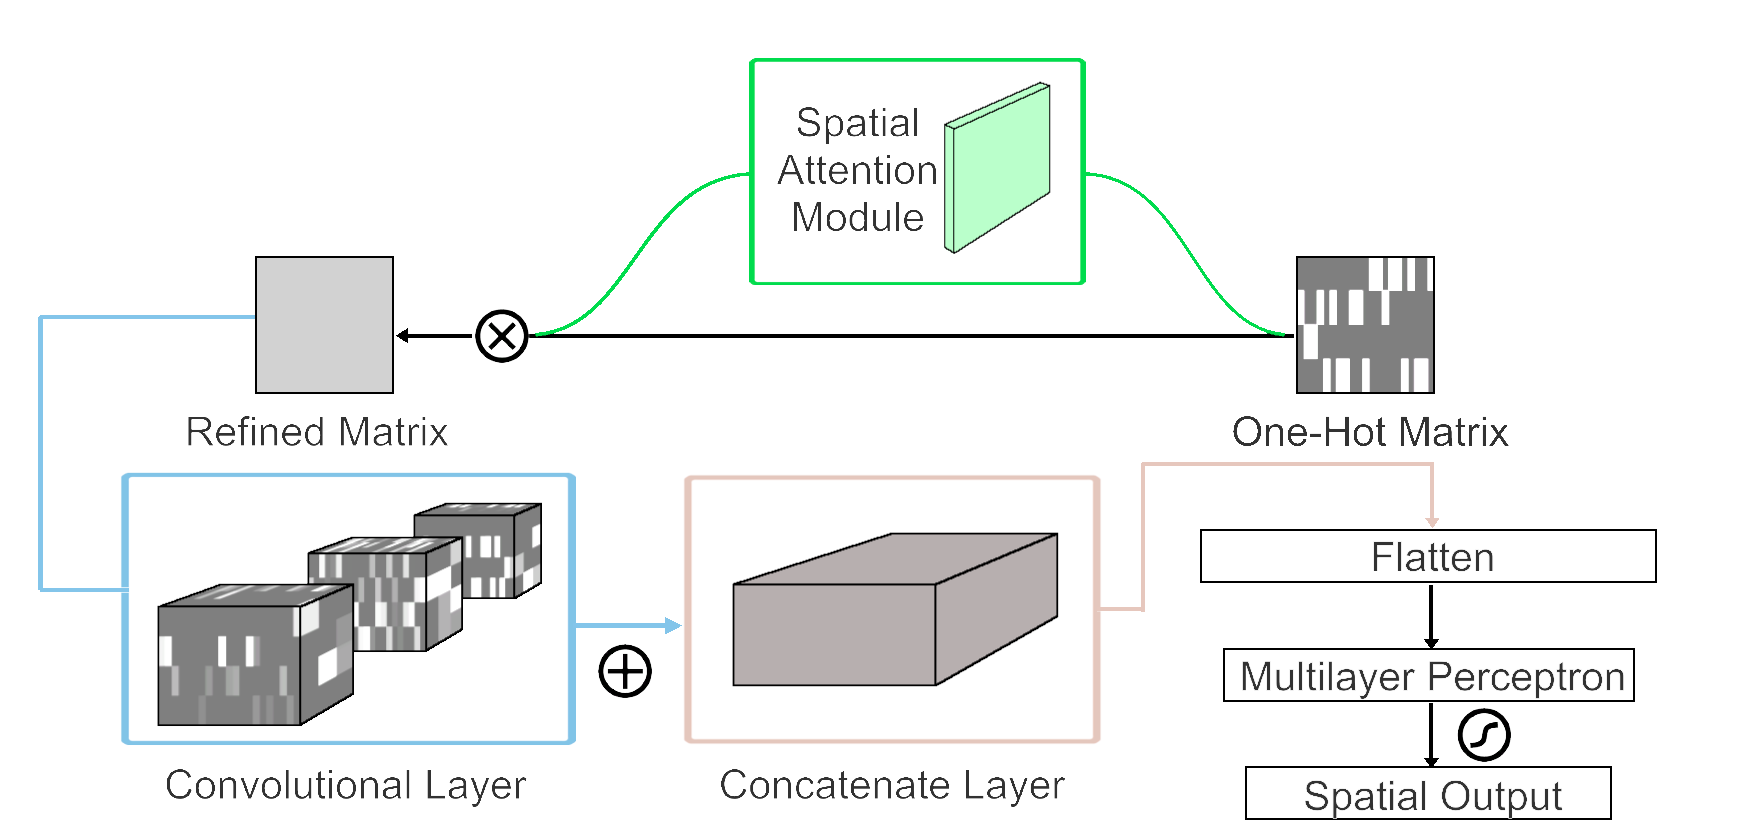
\includegraphics[width=86mm]{CNNv2.png}}
    \caption{The architecture of spatial domain method in AttCRISPR. 
    The input of the method is encoded sgRNA sequence, a $21\times 4$ one-hot matrix. 
    Then refine it through a spatial attention module, which could tell us the importance of a specific matrix element (or just say, pixel).
    Finally, a simple convolutional neural network is applied.}\label{fig:02}
\end{figure}
As Figure~2\vphantom{\ref{fig:02}} show, method in spatial domain relies on the convolutional neural network. 
As previously mentioned, sgRNA sequence has been encoded into a $21\times 4$ one-hot matrix $X_{oh}$, and we regard $X_{oh}$ as a binary image. 
Then, convolution kernels with different size are used to extract potential spatial features just like what other do in computer vision. 
According to the foregoing, the Spatial Attention Module proposed by \citeauthor{woo2018cbam:} can be applied in our method in spatial domain, 
which was used to improve the performance of CNN in vision tasks.

\begin{figure}[!tpb]%figure3
    \centerline{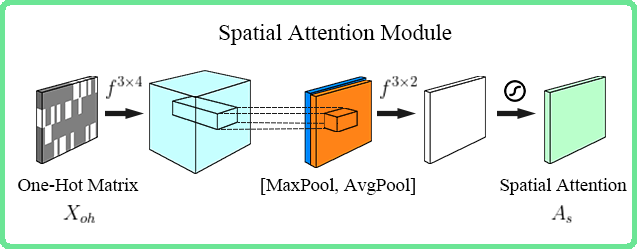
\includegraphics[width=86mm]{spatialmodule.png}}
    \caption{Details of spatial attention module. A convolution layer is used to generate multi-channel map from $X_{oh}$.
    Then concatenated the output of both max-pooling and average-pooling method and forward it to the last convolution layer.
    A sigmoid is used to map the final result to a range of zero to one.
    }\label{fig:03}
\end{figure}

As Figure~3\vphantom{\ref{fig:03}} show, Given an one-hot map $X_{oh}$, spatial attention module generating spatial attention matrix 
$A_s\in\mathbb{R}^{l\times 4}$ with the same as $X_{oh}$ in shape. 
Each element of $A_s$ is constrained to a range of zero to one, implemented by a sigmoid function, which reflects the importance of the corresponding elements of $X_{oh}$.
The overall spatial attention process can be summarized as:
\begin{equation}
\left\{\begin{matrix}
X_{mc} = f^{3\times4}(X_{oh})
\\A_s = \sigma(f^{3\times2}([AvgPool(X_{mc});MaxPool(X_{mc})]))
\\X_{rf} = A_s\otimes X_{oh}
\end{matrix}\right.\label{eq:11}
\end{equation}
where $f^{p\times q}$ represents a convolution operation with the filter size of $p\times q$, 
$p,q\in\mathbb{Z}^{+}$, $X_{mc}$ is a multi-channel map generated by $X_{oh}$, $\sigma$ denotes the sigmoid function, 
AvgPool denotes the average-pooling operation, MaxPool denotes the max-pooling operation, $\otimes$ denotes element-wise multiplication.
\begin{figure}[!tpb]%figure4
    \centerline{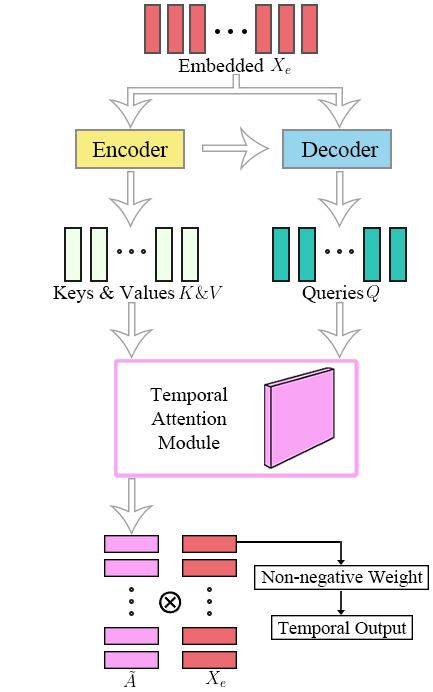
\includegraphics[width=86mm]{temporalmodule.png}}
    \caption{The architecture of temporal domain method in AttCRISPR. 
    The input of the method is embedding sgRNA sequence, a $21\times e$ embedding matrix, where $e$ is the dimension of a nucleotide embedding vector. 
    }\label{fig:04}
\end{figure}
Spatial attention matrix $A_s$ formally conforms to our proposed definition of first-order preference (each element of $X_{oh}$ is multiplied by the corresponding element of $A_s$), 
in other word, element of $A_s$ reveal how important the corresponding elements in $X_{oh}$ is. 
We think it can reveal the preference of the scoring function at each position. 
For instance, follow the encoding rules above, train spatial domain part of AttCRISPR with the WT-SpCas9 dataset. 
Then take the average of all spatial attention matrix, and the element in the first row and third column are closer to 1, which means when calculate the final score, 
G typically may have a important contribution at first position within sgRNA sequence. 
In fact, this corresponds to some early studies concerning the Human (hU6) promoter, which is believed to require G as the first nucleotide of its transcript \citep{cong2013multiplex,jinek2012a,mali2013rnaguided}.
\subsubsection{Method and attention in temporal domain}

\begin{figure}[!tpb]%figure3
    \centerline{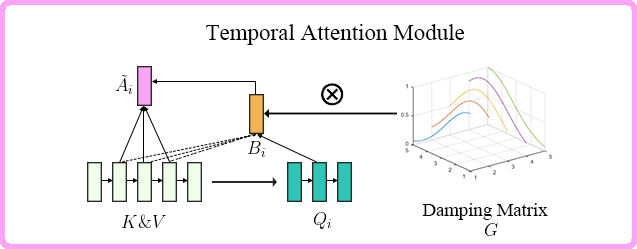
\includegraphics[width=86mm]{temporalattentionmodule.png}}
    \caption{wait2write
    }\label{fig:03}
\end{figure}
As Figure~4\vphantom{\ref{fig:04}} show, temporal domain part of AttCRISPR relies on the recurrent neural network (or its variant). 
As previously mentioned, we mapping each one-hot vector into a dense real-valued high-dimensional space follow the Equation~(\ref{eq:08}), which generates the embedded matrix $X_e$.
And we regard $X_{e}$ as a sequential data, or temporal data.
Recurrent neural network (or its variant) has showed outstanding performance in the tasks with temporal data (for instance, natural language processing, sequential recommendation). 
That's why we prefer to use it to extract potential temporal features. 
To be precise, we prefer the architecture of encoder-decoder which has been proven to be effective in Seq2Seq task. 
Two main differences we have to face are that sgRNA is not a natural language in the traditional sense, and we don't have to translate it to other sequence. 
To accommodate them, the embedded matrix $X_e$ is used as input of both the encoder and decoder, and the sequence of decoder is to build the first-order preference of sgRNA sequence $\tilde{A}$. 
As mentioned above, the predicted value $y$ should satisfy Equation~(\ref{eq:05}). 
On this basis, we apply the idea of attention mechanism which has been widely used in natural language processing tasks to AttCRISPR in the method of temporal domain, 
and name it Temporal Attention Module \citep{vaswani2017attention,luong2015effective,bahdanau2014neural}.
As the idea of \citeauthor{vaswani2017attention}, Temporal Attention Module satisfies the following equation
\begin{equation}
Attention(Q,K,V)=align(Q,K)V\label{eq:13}
\end{equation}
where the $align(\cdot)$ is put forward by \citeauthor{luong2015effective}. 
$Q$, $K$, $V$ are queries, keys and values matrix accordingly in the paper of \citeauthor{vaswani2017attention}. 
As Figure~5\vphantom{\ref{fig:05}} show, in our attention module they are calculated by the following equation
\begin{equation}
\left\{\begin{matrix}
K_i=Encoder({X_e}_i,\theta_E,K_{i-1})
\\ Q_i=Decoder({X_e}_i,\theta_D,Q_{i-1})
\\V=K 
\end{matrix}\right.\label{eq:14}
\end{equation}
where vector $K_i$, $Q_i$ denotes the $i$-th row of the matrix $K$ and $Q$ accordingly, $Encoder(\cdot)$ and $Decoder(\cdot)$ are independent GRU units, $\theta_E$ and $\theta_D$ denote all the related parameters of GRU networks accordingly. 
In the actual implementation, we apply the bidirectional GRU networks for better performance, and for the sake of conciseness, we show a conventional GRU network here. 
The function $align(\cdot)$ is as follows
\begin{equation}
B=align(Q,K)\label{eq:16}
\end{equation}
\begin{equation}
B_i=softmax(Q_iK^T)\otimes G_i\label{eq:17}
\end{equation}
\begin{equation}
G_{ij}=\left\{\begin{matrix}
exp(\frac{(i-j)^2}{-2\sigma})&,\left | i-j \right |\leqslant \sigma
\\ 0&,\left | i-j \right |>  \sigma
\end{matrix}\right.\label{eq:18}
\end{equation}
where the matrix $B\in\mathbb{R}^{l\times l}$ is the second-order preference we need, and vector $B_i$ denotes the $i$-th row of the matrix $B$. 
$G\in\mathbb{R}^{l\times l}$ is the damping matrix base on Gaussian function. 
Since a simple belief that the closer the base is to the $i$-th position, the more it affects the $i$-th position normally, we use the damping matrix G to constrain the network learning. 
$\sigma$ represents a threshold of length, any base over this length from the position $i$ is not considered to be affected.
Further, if we think of the values matrix as a vector form of the first-order preference $A$ in Equation~(\ref{eq:05}), we can reach the following equation
\begin{equation}
\tilde{A}=BV\label{eq:19}
\end{equation}
according to above, values matrix $V$ comes from the hidden states of a bidirectional GRU networks, which is usually hard to understand and explain.
While $B$ is the second-order preference matrix obtained by the attention mechanism, in our belief, the $j$-th dimension of $B_i$, denoted as $B_{ij}$, can reveal the effect of the base at position $j$ on position $i$ in the biological sense. 
\subsubsection{Model ensemble following stacking strategy}

Text

\subsection{Datasets and current prediction method}

text

\subsection{Experiments}

text

\section{Results}

Text

\enlargethispage{6pt}

Text

\subsection{Test1}

Text Text  Text

\section{Discussion}

Text

\section{Conclusion}

(Table~\ref{Tab:01}) Text Text Text Text Text Text  Text Text Text
Text Text Text Text Text Text  Text Text Text Text Text Text.

\section*{Acknowledgements}

Text
\begin{table}[!t]
    \processtable{This is table caption\label{Tab:01}} {\begin{tabular}{@{}llll@{}}\toprule head1 &
    head2 & head3 & head4\\\midrule
    row1 & row1 & row1 & row1\\
    row2 & row2 & row2 & row2\\
    row3 & row3 & row3 & row3\\
    row4 & row4 & row4 & row4\\\botrule
    \end{tabular}}{This is a footnote}
\end{table}
    
\vspace*{-12pt}

\section*{Funding}

This work has beenText  Text Text.\vspace*{-12pt}

\bibliographystyle{natbib}
%\bibliographystyle{achemnat}
%\bibliographystyle{plainnat}
%\bibliographystyle{abbrv}
%\bibliographystyle{bioinformatics}
%
%\bibliographystyle{plain}
%
\bibliography{document}

\end{document}